\documentclass{article}
\usepackage[UTF8]{ctex}
\usepackage{appendix}
\usepackage{graphicx} % Required for inserting images
\usepackage{amsmath}
\usepackage{listings}
\lstset{language=Python}  % 设置默认语言为Python

\begin{document}
\thispagestyle{empty}

\begin{figure}[t]
    \centering
    
\includegraphics[width=12cm]{logo2.png}
\end{figure}

\vspace*{\fill}
    \begin{center}
        \Huge\textbf{底盘线圈磁场仿真}
    \end{center}
\vspace*{\fill}

\begin{table}[b]
    \centering
    \large
    \begin{tabular}{ll}
    \textbf{院系:} & 电子信息与通信 \\
    \textbf{专业班级:} & 提高2101班 \\
    \textbf{姓名:} & 杨筠松 \\
    \textbf{学号:} & U202115980 \\
    \textbf{指导老师:} & 田加胜 \\
    \textbf{时间:} & 2023年12月\\
    \end{tabular}
\end{table}

\newpage
\pagenumbering{Roman}
\setcounter{page}{1}
\tableofcontents
\newpage
\setcounter{page}{1}
\pagenumbering{arabic}

\section{线圈模型与结构尺寸}
根据学号的顺序,我们需要研究和仿真的是第8号线圈——底盘线圈,具体形状如下图所示:


\begin{figure}[h]
  \centering
  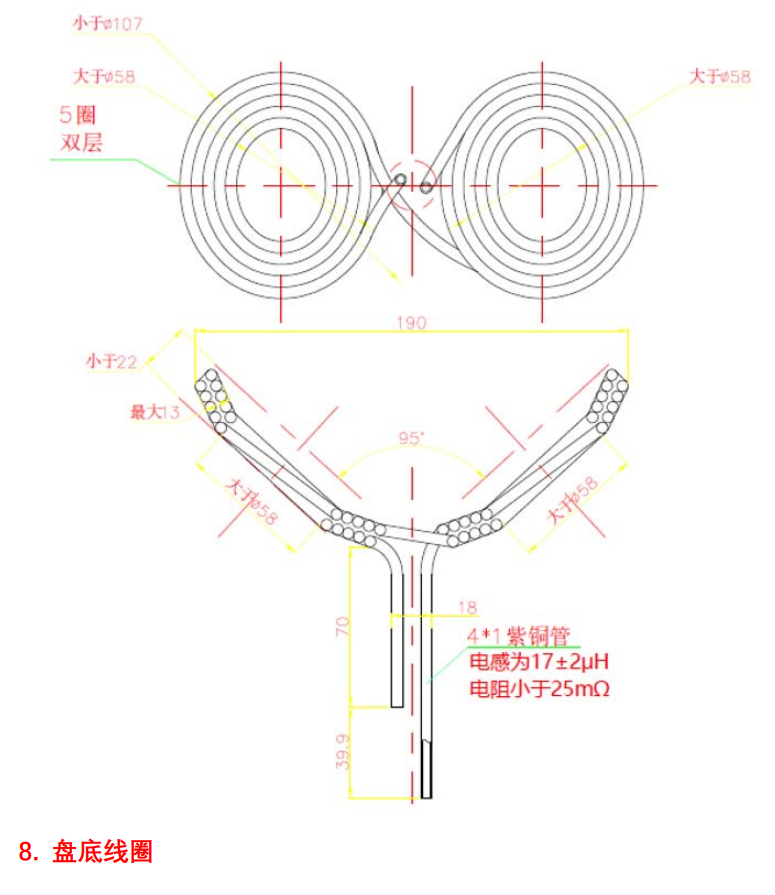
\includegraphics[scale=0.4]{constr.png}
  \caption{底盘线圈模型与结构尺寸}
  \label{fig:example}
\end{figure}
\newpage

\section{算法表达式与具体计算步骤}
\subsection{对载流圆环产生的磁场进行数学建模}
设载流圆环的半径为$R$, 其中通有电流为$I$。 如下图所示, 设载流圆环位于 $y-z$ 平面上, 圆心与坐标原点重合, 载流圆环中心轴线与 $x$ 轴重合。

\begin{figure}[h]
  \centering
  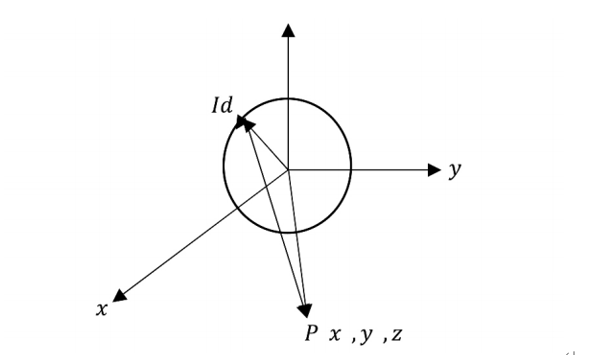
\includegraphics[scale=0.4]{coil.png}
  \caption{载流圆环磁场分析图}
  \label{fig:example}
\end{figure}

在空间任取一点 \(P(x_0, y_0, z_0)\),计算 \(P\) 处的磁感应强度。在圆环上任取电流元 \(Id\vec{l}\), 由毕奥 - 萨伐尔定律知该电流元在 \(P\) 点产生的磁感应强度为
\[
d\vec{B} = \frac{\mu_0}{4\pi} \frac{I(d\vec{l}) \times \vec{r}}{r^3}
\]
其中 \(\vec{r}\) 为电流元到 \(P\) 点的距离。
由磁场的叠加原理, 则 \(P\) 点的磁感应强度为
\[
\vec{B} = \oint_C \frac{\mu_0}{4\pi} \frac{I(d\vec{l}) \times \vec{r}}{r^3}
\]
因为直接求取该积分计算过程复杂且易出错, 所以为了简化计算过程, 我们在空间直角坐标系中, 首先分别求取在 \(x\) 轴, \(y\) 轴, \(z\) 轴的磁感应强度分量, 然后求矢量和得 \(P\) 点的磁感应强度, 最后绘制磁场分布图, 分析载流圆环在全空间的磁场分布特点。

设 \((x, y, z)\) 为电流元的坐标, 则电流元 \(I d\vec{l}\) 和电流元到 \(P\) 点的距离 \(\vec{r}\) 在空间直角坐标系下的表示:
\[
d\vec{l} = dx\hat{i} + dy\hat{j} + dz\hat{k}, \quad \vec{r} = (x_0-x)\hat{i} + (y_0-y)\hat{j} + (z_0-z)\hat{k}
\]

将式(2)(3)代入式(1), 其中
\[
\begin{aligned}
    d\vec{l} \times \vec{r} &= \begin{vmatrix}
        \hat{i} & \hat{j} & \hat{k} \\
        dx & dy & dz \\
        (x_0-x) & (y_0-y) & (z_0-z)
        \end{vmatrix} \\
        &= ((z_0-z)dy - (y_0-y)dz)\hat{i} + ((x_0-x)dz - (z_0-z)dx)\hat{j} \\
        &\quad + ((y_0-y)dx - (x_0-x)dy)\hat{k}
\end{aligned}
\]

所以 \(P\) 点的磁感应强度分量为:
\[
\begin{aligned}
    B_x &= \oint_C \frac{\mu_0 I}{4\pi} \frac{((z_0-z)dy - (y_0-y)dz)}{r^3}, \\
    B_y &= \oint_C \frac{\mu_0 I}{4\pi} \frac{((x_0-x)dz - (z_0-z)dx)}{r^3}, \\
    B_z &= \oint_C \frac{\mu_0 I}{4\pi} \frac{((y_0-y)dx - (x_0-x)dy)}{r^3}
\end{aligned}
\]

于是得到了一个载流环的磁场分布。

\subsection{对2D螺旋线圈产生的磁场进行建模}
在上面的一节讨论中,我们清楚了只要给定一个电流元的坐标,那么他对空间中任意一点$P(x_0, y_0, z_0)$的磁感应强度均可计算得到,那么现如今问题在于如何仿真螺旋线圈并且半径正在不断变化的情况呢,如果我们可以确定线圈上任何一点的坐标,那么其产生的磁感应强度便随之迎刃而解了,具体结构如下图所示:

\begin{figure}[h]
  \centering
  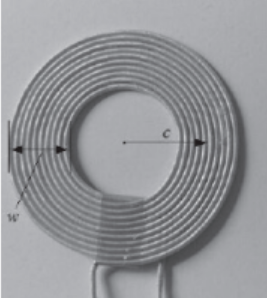
\includegraphics[scale=0.4]{constr2.png}
  \caption{螺旋线圈结构}
  \label{fig:example}
\end{figure}

我们有如下假设和约定:考虑线圈圆心位于$y-z$平面上,为$s_0 = (0, -m, m)$,设$r_0$表示螺旋线圈开始的半径长度,$\beta$为每一圈螺线增加的半径,$N$为总共螺线圈数,螺线圈自身材料半径忽略不计,线圈所在平面同$x-y$平面夹角为$\alpha$,那么对于给定给的角度$x(rad)$,此处$x\in[0, 10\pi]$,那么对应的坐标可由下面式子计算得到:
\[
\begin{aligned}
    r' &= r_0 + \frac{x\beta}{2\pi}\\
    x_{new} &= s_{0_x} + r'sinx \\
    y_{new} &= s_{0_y} + r'cosxsin\alpha\\
    z_{new} &= s_{0_z} + r'cosxcos\alpha
\end{aligned}
\]

那么此时便可以利用新得到的坐标$(x_new, y_{new}, z_{new})$来计算空间中任何一点$P(x, y, z)$的磁场分布。


\newpage



\section{Python程序代码运行结果分析}

\subsection{模型验证}
首先我们需要对之前的二维螺线圈进行验证,运行verify1.py得到如下图所示:

\begin{figure}[h]
  \centering
  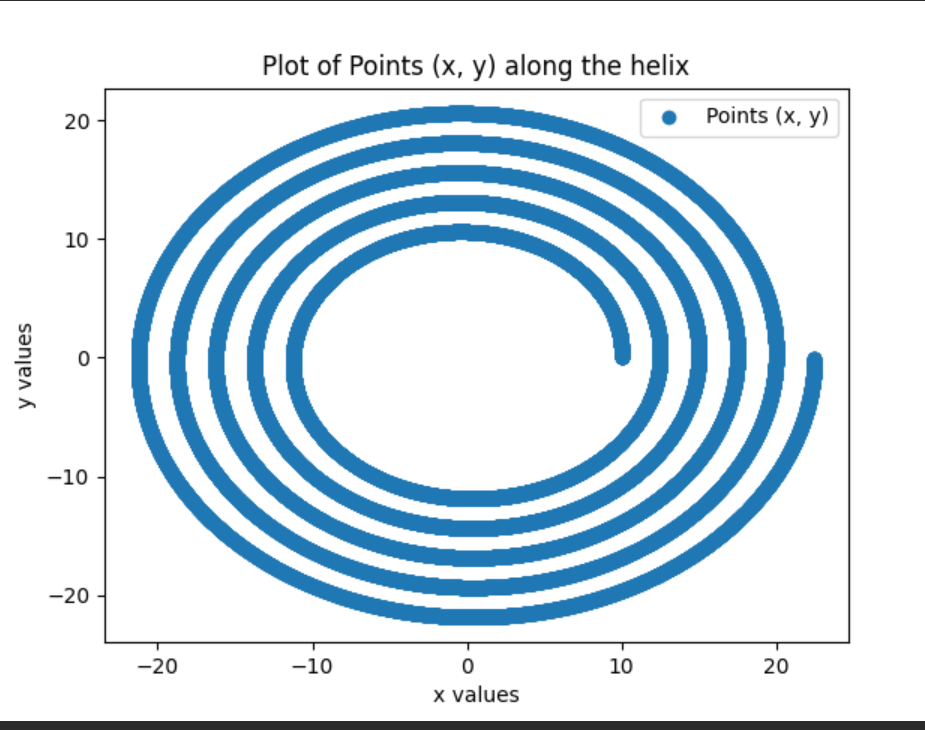
\includegraphics[scale=0.2]{veri1.png}
  \caption{2d螺旋线圈}
  \label{fig:example}
\end{figure}
其中设置参数为$\beta= 2.5mm/turn$, $N=5$, 现如今将它放入到三维空间中来保证后续仿真的正确性,运行verify.py文件得到下图

\begin{figure}[h]
  \centering
  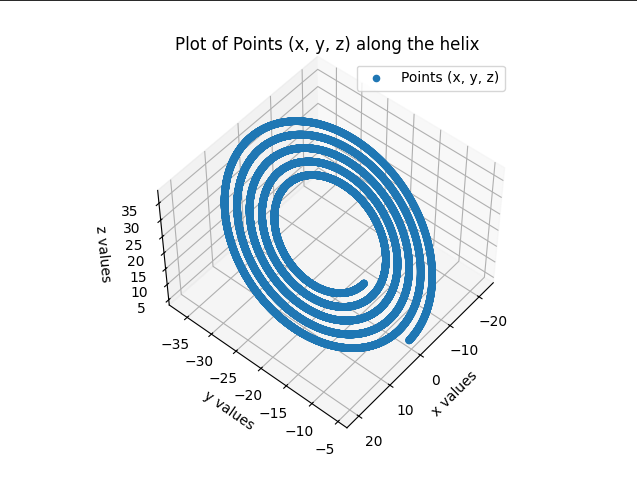
\includegraphics[scale=0.35]{veri2.png}
  \caption{3d螺旋线圈结果}
  \label{fig:example}
\end{figure}

如此可以说明,上述对于螺线线圈的的模型建立是正确的。

\subsection{具体仿真结果}
运行main.py文件可以得到如下的三张图片,分别代表着
当$z = 0$时,只展示xy平面:

\begin{figure}[h]
  \centering
  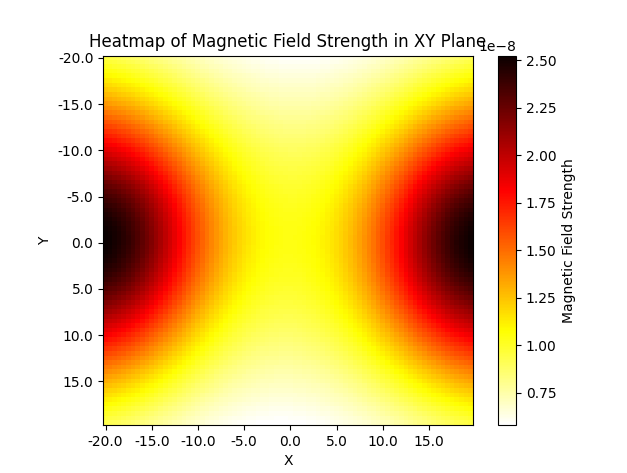
\includegraphics[scale=0.35]{results/result1.png}
  \caption{xy平面仿真结果}
  \label{fig:example}
\end{figure}

当$y=0$,只展示$xz$平面:

\begin{figure}[h]
  \centering
  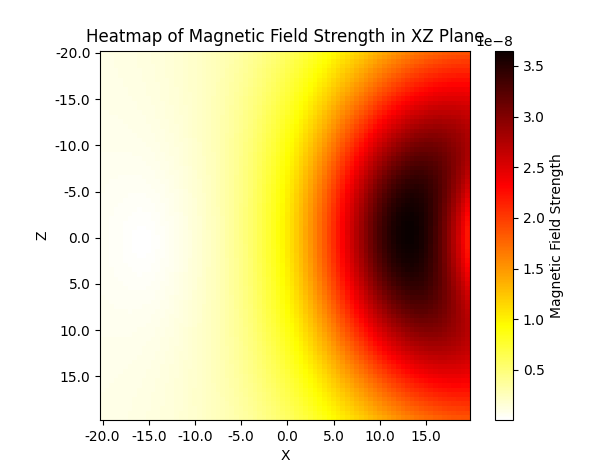
\includegraphics[scale=0.35]{results/result2.png}
  \caption{xz平面仿真结果}
  \label{fig:example}
\end{figure}

当$x = 0$时,只展示$yz$平面

\begin{figure}[h]
  \centering
  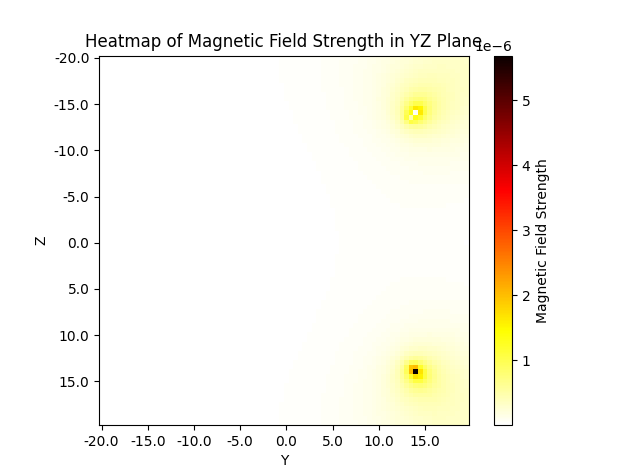
\includegraphics[scale=0.35]{results/result3.png}
  \caption{yz平面仿真结果}
  \label{fig:example}
\end{figure}

全部都使用热力图来进行表示,使得结果更加直观,排除了3d视觉差效果造成的影响。

\section{Ansys Maxwell 软件仿真结果}
\subsection{仿真模型建立}
观察模型,可以发现把手本身的磁效应并不会对整体结果造成影响,故而可以进行简化,而由于电脑的配置问题,运行两层5圈对称的线圈将会使得电脑运行周期过长,并且结果难以进行观察,遂降模型简化成如下图所示,仅有一层但是有良好可分析性:

\begin{figure}[h]
  \centering
  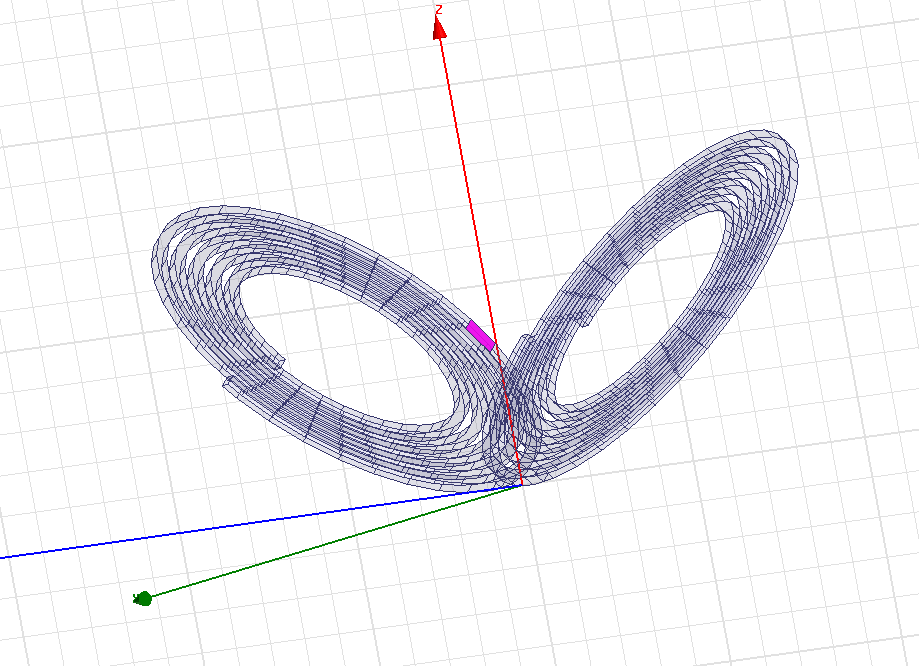
\includegraphics[scale=0.25]{procedure/base.png}
  \caption{模型创建}
  \label{fig:example}
\end{figure}\textbf{}

我们可以进行如下的线圈参数设置:

\begin{figure}[h]
  \centering
  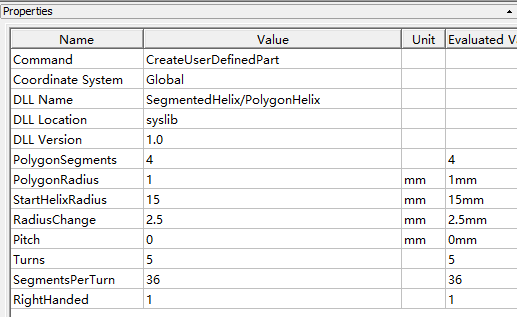
\includegraphics[scale=0.4]{procedure/property.png}
  \caption{线圈参数}
  \label{fig:example}
\end{figure}\textbf{}

同时依次设立边界(其余四面不再一一列出),激励电流,以及求解器类型如下:

\begin{figure}[h]
  \centering
  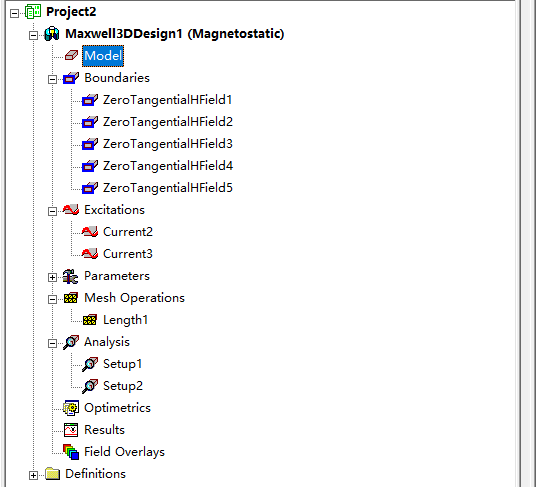
\includegraphics[scale=0.3]{procedure/helper.png}
  \caption{项目管理器}
  \label{fig:example}
\end{figure}\textbf{}

\begin{figure}[h]
  \centering
  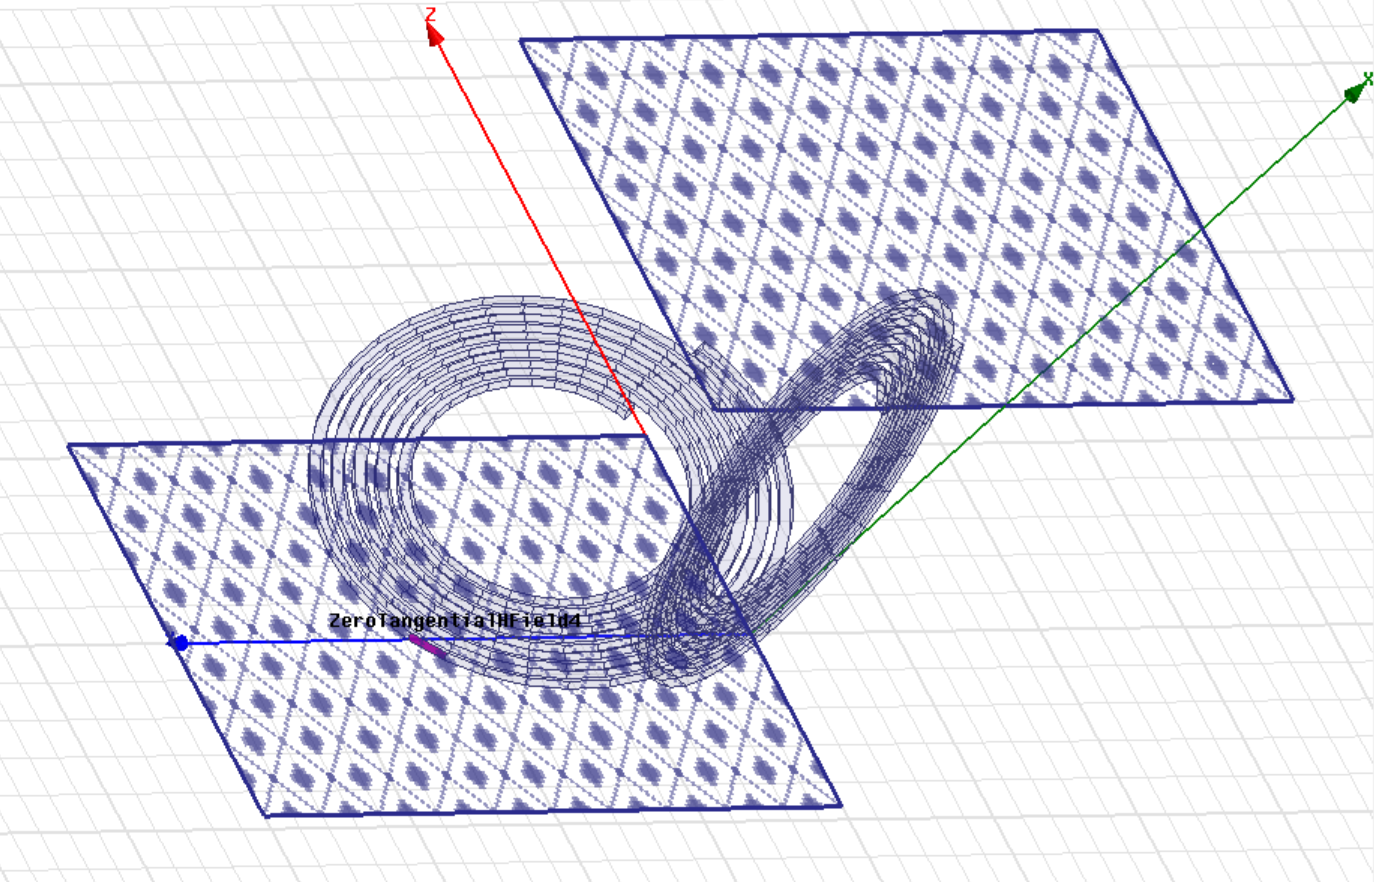
\includegraphics[scale=0.18]{procedure/bounder.png}
  \caption{边界}
  \label{fig:example}
\end{figure}\textbf{}

\begin{figure}[h]
  \centering
  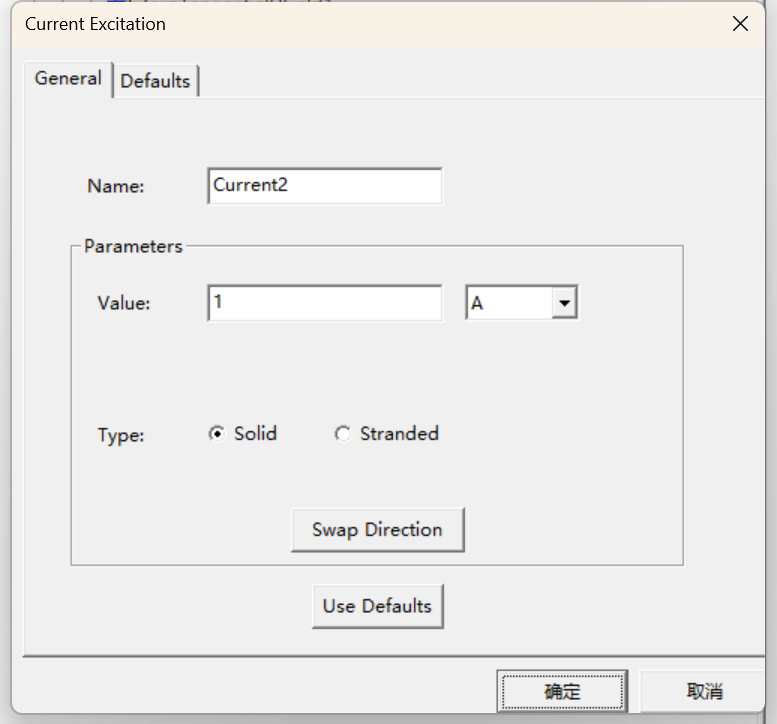
\includegraphics[scale=0.2]{procedure/current.png}
  \caption{激励电流}
  \label{fig:example}
\end{figure}\textbf{}

选择求解器为静电场即可,此时并不需要考虑边际效应,因为本身的影响较小。


\subsection{仿真结果展示}
在仿真之前需要对模型进行认证,防止出现无法运行的错误,需要点击Validation check,所有验证均通过后,便可选择Analyse all,进行模型求解,得到如下的三个平面上的$B$热力图,如下所示,注意矩阵的设置和选择,并且执行Field Overlays需要选取一个平面(plane)进行分析,不能选择物体(object),否则将会明显报错。

\newpage
\textbf{$XY$平面}

\begin{figure}[h]
  \centering
  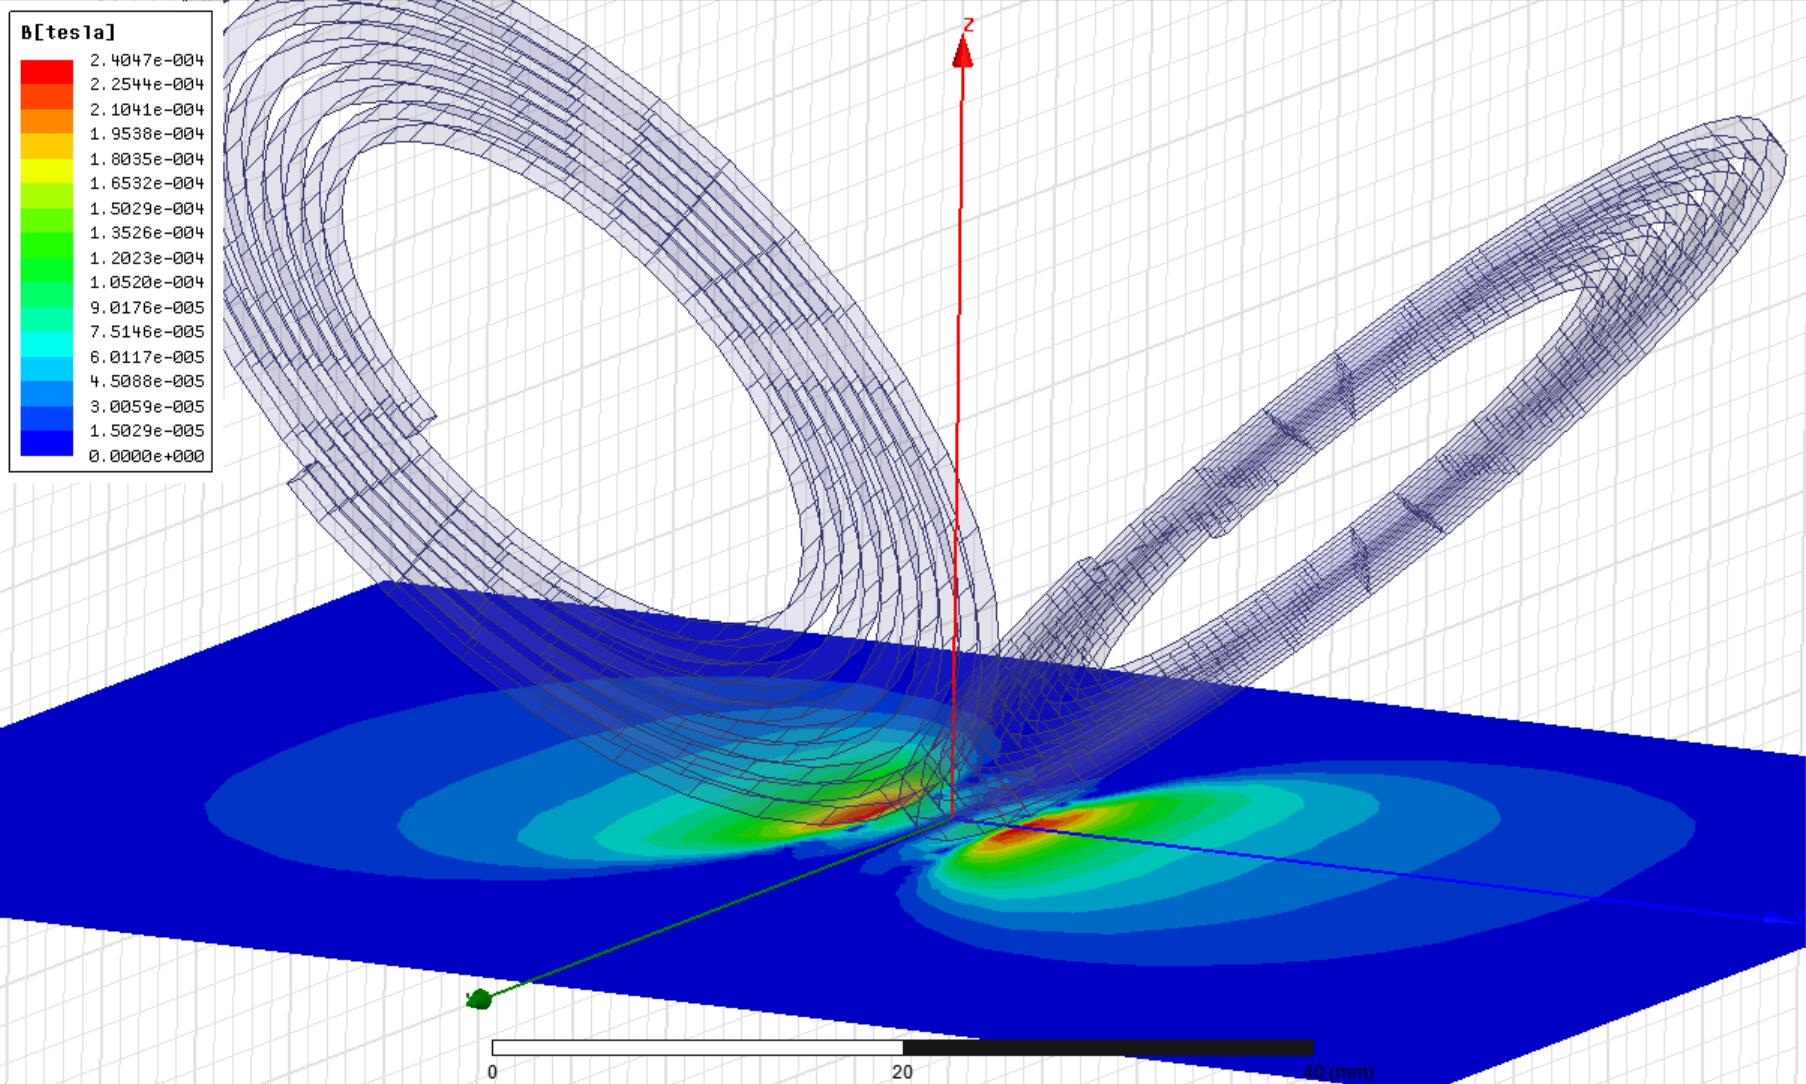
\includegraphics[scale=0.2]{simulation/res1.jpg}
  \caption{XY plane}
  \label{fig:example}
\end{figure}\textbf{}

\textbf{$XZ$平面}

\begin{figure}[h]
  \centering
  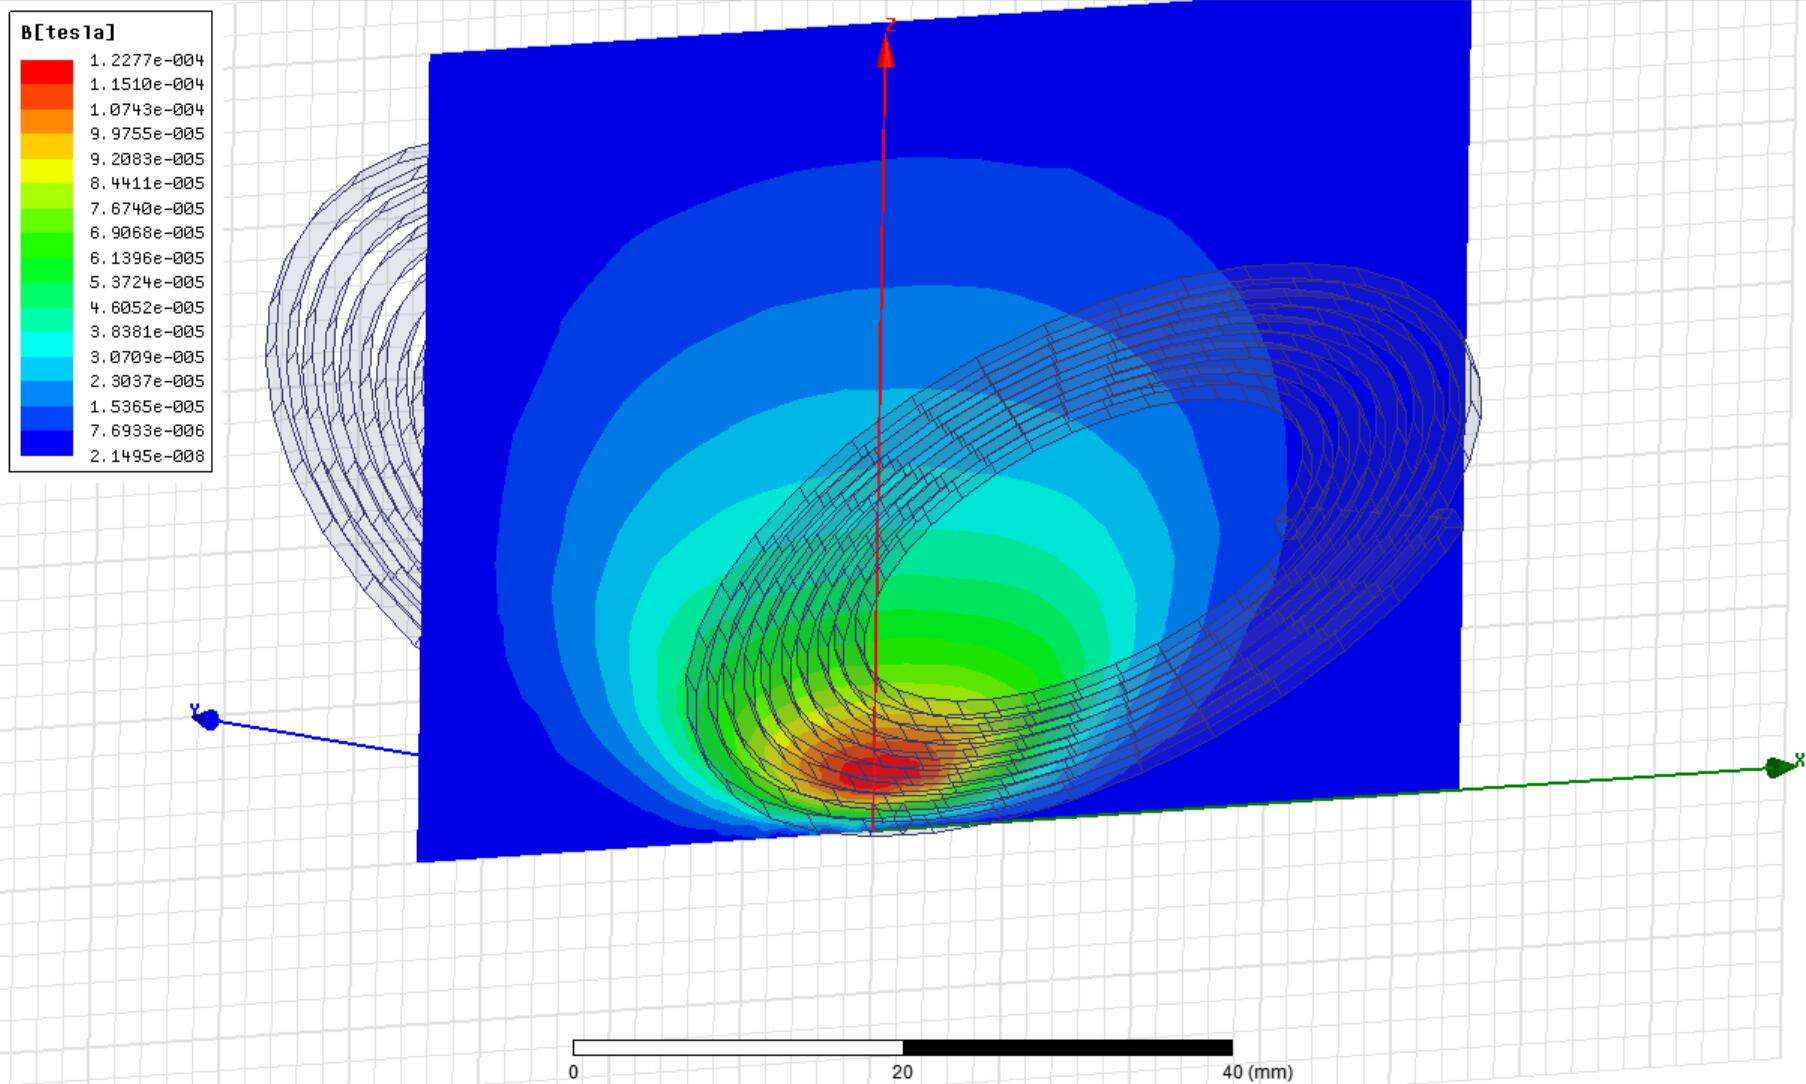
\includegraphics[scale=0.2]{simulation/res2.jpg}
  \caption{XZ plane}
  \label{fig:example}
\end{figure}\textbf{}

\textbf{$YZ$平面}

\begin{figure}[h]
  \centering
  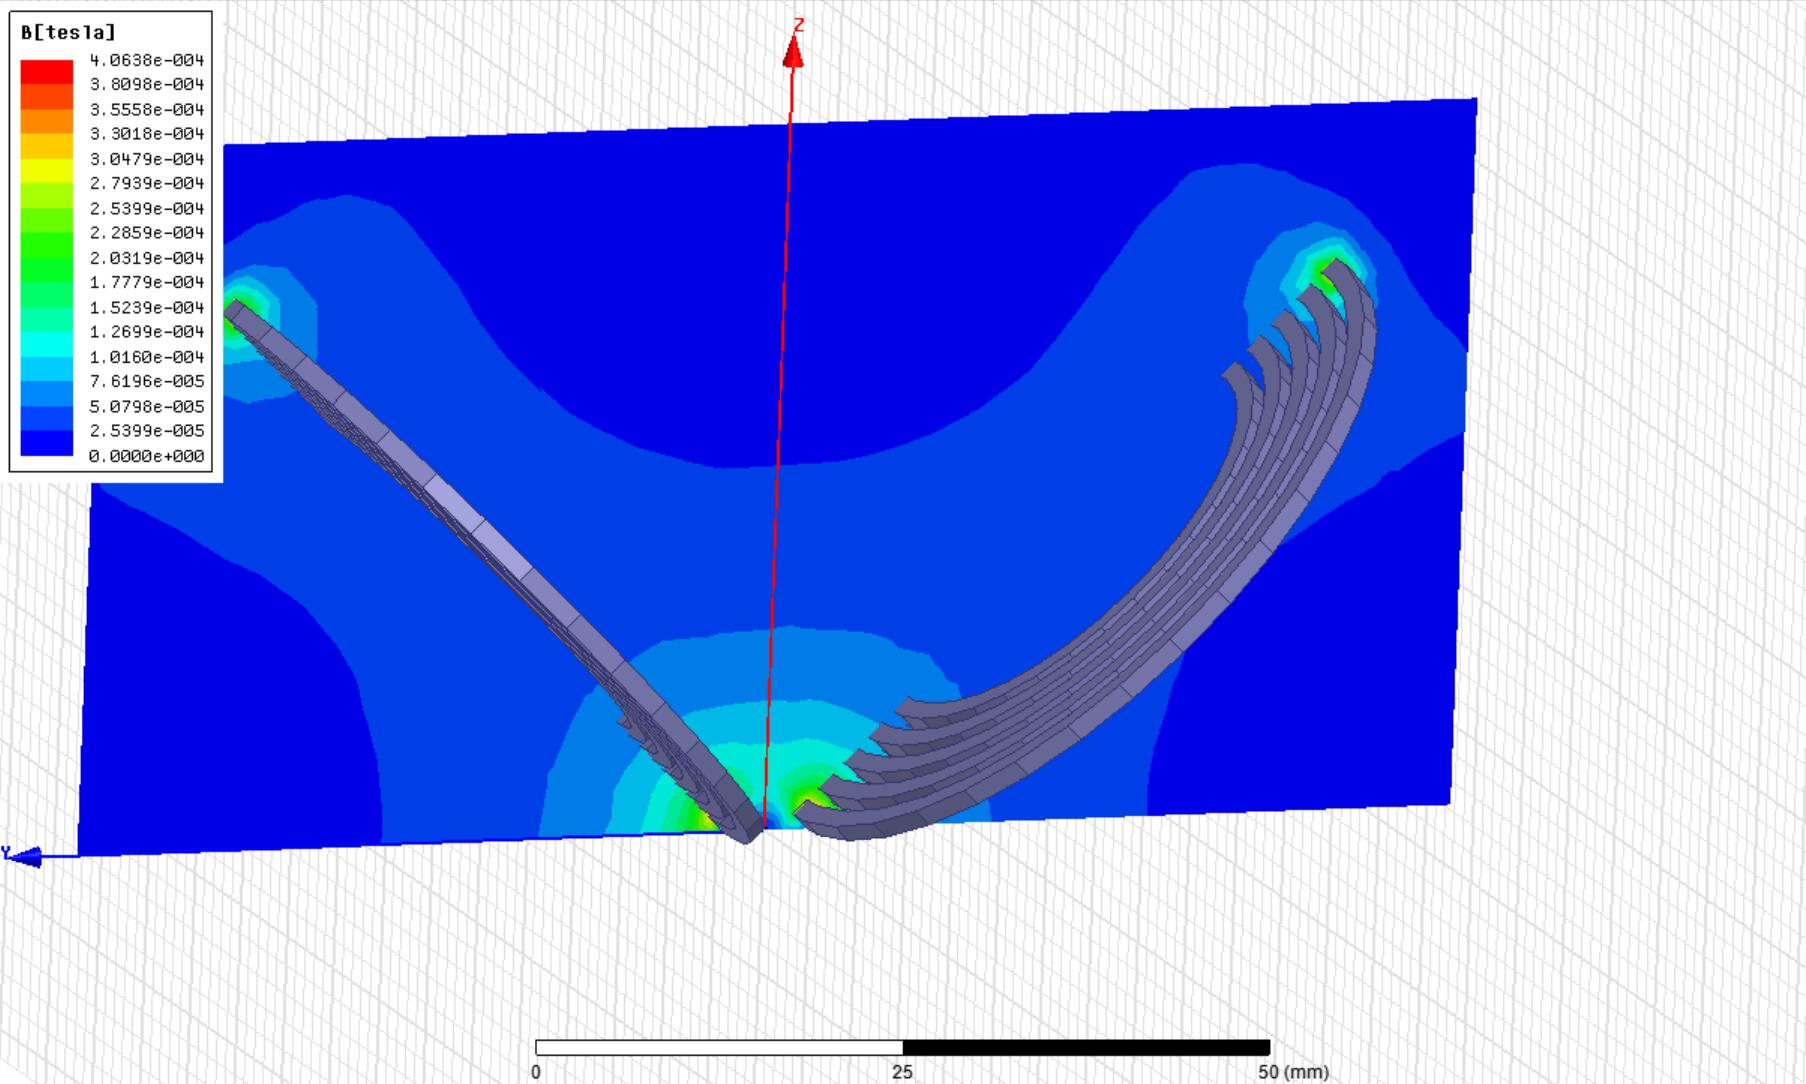
\includegraphics[scale=0.2]{simulation/res3.jpg}
  \caption{YZ plane}
  \label{fig:example}
\end{figure}\textbf{}



\section{结果分析与对比}
观察python仿真的热力图和Ansys Maxwell仿真结果,对于xy平面,可以发现呈现出中轴对称的形式,二者结果一致,对于xz平面,可以发现靠近原点的到X轴正半轴方向逐渐加大,但是碍于图片大小限制,无法完整展现又最大变到最小的过程,但是基本符合事实。对于yz平面,两点型特征极具辨识度,有效的展现了此时的磁场变化特征。

综上所述,本次仿真python代码和Ansys Maxwell软件基本一致,实验内容较为完善。

\begin{appendices}
    \renewcommand{\thesection}{\Alph{section}}
    \section{verify.py}

    \begin{lstlisting}
import numpy as np
import matplotlib.pyplot as plt
from mpl_toolkits.mplot3d import Axes3D

# define the basic variables
m = 27.5 / np.sqrt(2) + 2
pi = 3.1415926
s0, s1 = [0, -m, m], [0, m, m]
alpha0, alpha1 = 3 / 4 * pi, 1 / 4 * pi
startHelix = 10
radiusChange = 2.5
turns = 5

def calculateB(x, y, z, elev=None, azim=None):
    x_values, y_values, z_values = [], [], []
    for x_val in np.arange(0, 10 * np.pi, 0.001):
        rPrime = calculateRPrime(x_val)
        x_new = s0[0] + rPrime * np.sin(x_val)
        y_new = s0[1] + rPrime * np.cos(x_val) * np.sin(alpha0)
        z_new = s0[2] + rPrime * np.cos(x_val) * np.cos(alpha0)
        x_values.append(x_new)
        y_values.append(y_new)
        z_values.append(z_new)

    # Plot the values for verifying
    fig = plt.figure()
    ax = fig.add_subplot(111, projection='3d')

    if elev is not None and azim is not None:
        ax.view_init(elev=elev, azim=azim)

    ax.scatter(x_values, y_values, z_values, label='Points(x,y,z)')
    ax.set_xlabel('x values')
    ax.set_ylabel('y values')
    ax.set_zlabel('z values')
    ax.set_title('Plot of Points (x, y, z) along the helix')
    plt.legend()
    plt.show()


def calculateRPrime(x):
    return startHelix + x * radiusChange / (2 * np.pi)


if __name__ == "__main__":
    calculateB(5, 0, 0, elev=50, azim=40) 
    \end{lstlisting}


    \section{main.py}

    \begin{lstlisting}
import numpy as np
import matplotlib.pyplot as plt
from matplotlib import cm
from matplotlib import axes
from matplotlib.font_manager import FontProperties
font = FontProperties(fname='/Library/Fonts/Songti.ttc')

# define the basic variables
m = 27.5 / np.sqrt(2) + 2
pi = 3.1415926
s0, s1 = [0, -m, m], [0, m, m]
alpha0, alpha1 = 3 / 4 * pi, 1 / 4 * pi
startHelix = 10
radiusChange = 2.5
turns = 5
mu = 4*np.pi * 1e-7
I = 1


def calculateB(x, y, z):
    tar = np.array([x, y, z])
    sumB = np.array([0.0, 0.0, 0.0])
    pre = None
    # calculate r_prime for all the cases
    r_prime_values = [calculateRPrime(x_val) for x_val 
        in np.arange(0, 10 * np.pi, 0.01)]

    for s in [s0, s1]:
        pre = None
        for x_val, rPrime in zip(np.arange(0, 10 * np.pi, 0.1),
                    r_prime_values):
            # calculate the position of new point
            x_new = s[0] + rPrime * np.sin(x_val)
            y_new = s[1] + rPrime * np.cos(x_val) 
                * np.sin(alpha0 if s == s0 else alpha1)
            z_new = s[2] + rPrime * np.cos(x_val) 
                * np.cos(alpha0 if s == s0 else alpha1)

            if pre is not None:
                cur = np.array([x_new, y_new, z_new])
                # calculate the vector dl
                dl = pre - cur

                # calculate the vector r and |r|^3
                r = cur - tar
                r_norm = np.linalg.norm(r) ** 3

                # calculate dl x r and sum them altogether
                demo_B = np.cross(dl, r)
                sumB += demo_B / r_norm

            pre = np.array([x_new, y_new, z_new])
    # return back
    return mu * I * np.linalg.norm(sumB) / (4 * np.pi)


def calculateRPrime(x):
    return startHelix + x * radiusChange / (2 * np.pi)



def simulateXY():
    x_values, y_values= np.arange(-20, 20, 0.5), 
            np.arange(-20, 20, 0.5)
    B_values = []
    for x in x_values:
        temp = []
        for y in y_values:
            temp.append(calculateB(x, y, 0))
        B_values.append(temp)
        print(x)
    fig = plt.figure()
    ax = fig.add_subplot(111)

    fig, ax = plt.subplots()
    im = ax.imshow(B_values, cmap=plt.cm.hot_r)

    x_ticks = np.arange(0, len(x_values), 10)
    y_ticks = np.arange(0, len(y_values), 10)

    ax.set_xticks(x_ticks)
    ax.set_xticklabels(x_values[x_ticks])
    ax.set_yticks(y_ticks)
    ax.set_yticklabels(y_values[y_ticks])

    cbar = plt.colorbar(im)
    cbar.set_label('Magnetic Field Strength')

    ax.set_xlabel('X')
    ax.set_ylabel('Y')
    ax.set_title('Heatmap of Magnetic Field Strength in XY Plane')

    plt.show()


def simulateXZ():
    x_values, z_values= np.arange(-20, 20, 0.5), 
            np.arange(-20, 20, 0.5)
    B_values = []
    for x in x_values:
        temp = []
        for z in z_values:
            temp.append(calculateB(x, 0, z))
        B_values.append(temp)
        print(x)
    fig = plt.figure()
    ax = fig.add_subplot(111)

    fig, ax = plt.subplots()
    im = ax.imshow(B_values, cmap=plt.cm.hot_r)

    x_ticks = np.arange(0, len(x_values), 10)
    y_ticks = np.arange(0, len(z_values), 10)

    ax.set_xticks(x_ticks)
    ax.set_xticklabels(x_values[x_ticks])
    ax.set_yticks(y_ticks)
    ax.set_yticklabels(z_values[y_ticks])

    cbar = plt.colorbar(im)
    cbar.set_label('Magnetic Field Strength')

    ax.set_xlabel('X')
    ax.set_ylabel('Z')
    ax.set_title('Heatmap of Magnetic Field Strength in XZ Plane')

    plt.show()


def simulateYZ():
    y_values, z_values= np.arange(-20, 20, 0.5), 
    np.arange(-20, 20, 0.5)
    B_values = []
    for y in y_values:
        temp = []
        for z in z_values:
            temp.append(calculateB(0, y, z))
        B_values.append(temp)
        print(y)
    fig = plt.figure()
    ax = fig.add_subplot(111)

    fig, ax = plt.subplots()
    im = ax.imshow(B_values, cmap=plt.cm.hot_r)

    x_ticks = np.arange(0, len(y_values), 10)
    y_ticks = np.arange(0, len(z_values), 10)

    ax.set_xticks(x_ticks)
    ax.set_xticklabels(y_values[x_ticks])
    ax.set_yticks(y_ticks)
    ax.set_yticklabels(z_values[y_ticks])

    cbar = plt.colorbar(im)
    cbar.set_label('Magnetic Field Strength')

    ax.set_xlabel('Y')
    ax.set_ylabel('Z')
    ax.set_title('Heatmap of Magnetic Field Strength in YZ Plane')

    plt.show()
    

if __name__ == "__main__":
    simulateXY()
    simulateXZ()
    simulateYZ()
        
         
    \end{lstlisting}
        
\end{appendices}



\end{document}
